\documentclass[a4paper, 11pt]{report}
\usepackage[utf8]{inputenc}   % Pour lire les fichiers UTF-8
\usepackage[T1]{fontenc}      % Pour une meilleure gestion des caractères accentués
\usepackage{textcomp}         % Pour quelques symboles supplémentaires
\usepackage{lmodern}          % Police compatible avec T1
\usepackage[english,french]{babel} 
\usepackage{graphicx} % Pour les images
\def\@captype{figure}
\usepackage{float}
\usepackage{multicol} % Pour faire des multi colonnes
\usepackage[export]{adjustbox} % Pour la clé 'valign'  (aligner verticalement)
\usepackage[colorlinks=true,linkcolor=black]{hyperref} % Pour qu'il y est des liens sur la table des matières
\usepackage{caption} % Utiliser plus de fonction sur caption (caption* pour ne pas afficher FIGURE-1)
\usepackage{lipsum} % Pour générer du texte pour voir comment ca rend
\usepackage{ragged2e} % Pour justifier le texte
\usepackage{ulem}
\usepackage[margin=3.2cm]{geometry}
\usepackage{forest}
\usepackage{listings}
\usepackage{xcolor}
\usepackage[section]{placeins}
\usepackage{amsmath}
\usepackage{amssymb}
\usepackage{fancybox}
\usepackage{fancyhdr}
\usepackage[none]{hyphenat}
\emergencystretch=3em
\usepackage{graphicx}
\usepackage{adjustbox}
\usepackage{float}


\usepackage{csquotes}


% Configuration de fancyhdr
\pagestyle{fancy}
\fancyhf{} % Efface tous les en-tètes et pieds de page précédents
\fancyhead[C]{Rapport de Projet} % Texte centré en haut de la page
\fancyfoot[L]{2025} % Texte en bas à  gauche du pied de page
\fancyfoot[C]{COUTANT, LITAMPHA, PETER} % Texte au centre du pied de page
\fancyfoot[R]{\thepage} % Numéro de page en bas à  droite du pied de page

\renewcommand{\headrulewidth}{0.4pt} % à‰paisseur de la ligne de séparation de l'en-tète
\renewcommand{\footrulewidth}{0.4pt} % à‰paisseur de la ligne de séparation du pied depage
\setlength{\headheight}{13.59999pt}
% Appliquer le style d'en-tète fancy aux pages de début de chapitre

\fancypagestyle{plain}{
  \fancyhf{} % Effacer tous
  \fancyhead[C]{Rapport de Projet} % Texte centré en haut de la page
  \fancyfoot[L]{L3 Informatique} % Texte en bas à  gauche du pied de page
  \fancyfoot[C]{COUTANT, LITAMPHA, PETER} % Texte au centre du pied de page
  \fancyfoot[R]{\thepage} % Numéro de page en bas à  droite du pied de page
  \renewcommand{\headrulewidth}{0.4pt} % à‰paisseur de la ligne de séparation de l'en-tète
  \renewcommand{\footrulewidth}{0.4pt} % à‰paisseur de la ligne de séparation du pied de page
}




\begin{document}

% Page de titre

% Page de titre
\begin{titlepage}
    \centering
    \vspace{3cm}
    \includegraphics[width=0.4\textwidth]{images/logo_univ.jpg}\hfill
    \includegraphics[width=0.5\textwidth]{images/logo_ufrst.png}\\
    \vspace{1.5cm}
    {\huge \textbf{Université Marie \& Louis Pasteur\\ UFR Sciences et Techniques}\par}
    \vspace{0.5cm}


    \shadowbox{\parbox{0.9\linewidth}{\centering \huge \textbf{Projet L3 : Pacman en réseau}}}\\
    \vspace{1cm}
    {\Large \textbf{Rapport de Projet} \\ Licence CMI Informatique - 3ème année \\ 2025-2026\par}
    \vspace{0.5cm}

    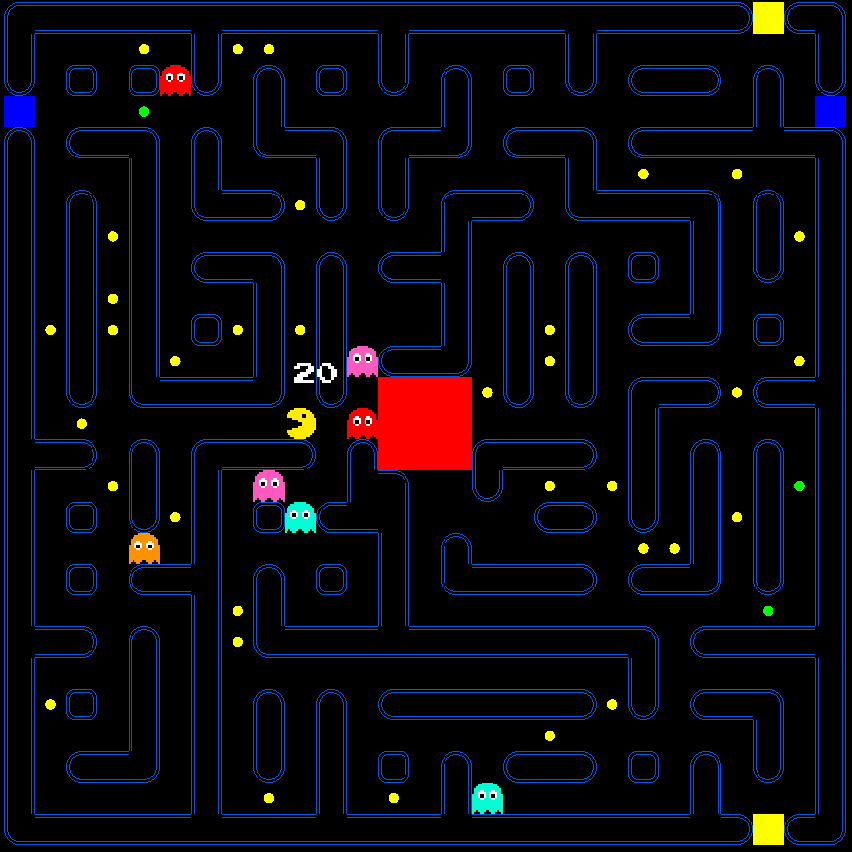
\includegraphics[width=0.7\textwidth]{images/entete.png}\\
    \vspace{0.5cm}

    {\LARGE \textbf{Thomas COUTANT}\\ \textbf{Benoît LITAMPHA}\\ \textbf{Auriane PETER}\par}
    \vspace{1cm}
    {\large \textbf{Encadrant : Julien BERNARD} }\\

    
\end{titlepage}


    


\chapter*{Remerciements}
\addcontentsline{toc}{chapter}{Remerciements}


\tableofcontents
\listoffigures

\chapter*{Introduction}
\addcontentsline{toc}{chapter}{Introduction}



\vfill


\chapter{Présentation du projet}

\section{Contexte académique}

Ce projet a été réalisé dans le cadre du semestre six de la licence informatique de l’Université Marie \& Louis Pasteur. Il s’inscrit dans un enseignement visant à mettre en pratique les connaissances acquises au cours de la formation, notamment à travers la réalisation d’un projet informatique de taille conséquente à plusieurs.

Le travail a été mené en groupe de trois étudiants sur une période s’étendant de la mi-octobre à la fin du mois de mars, sous l’encadrement de Julien Bernard, maître de conférences à l’Université Marie \& Louis Pasteur. Le projet porte sur le développement d’un jeu vidéo en réseau, de sa conception jusqu’à son implémentation.

Les objectifs pédagogiques de ce projet sont multiples. Il vise en particulier à consolider les compétences en programmation C++, à approfondir la découverte du développement de jeux vidéo, ainsi qu’à mettre en \oe uvre une architecture réseau de type client–serveur. Le projet permet également de développer des compétences transversales telles que le travail en équipe et la gestion d’un projet informatique sur une durée prolongée.

\section{Présentation générale du jeu \texttt{Pac-Man}}

Le jeu \texttt{Pac-Man}, apparu au début des années 1980, est un jeu d’arcade dans lequel le joueur contrôle un personnage évoluant dans un labyrinthe. L’objectif principal est de parcourir l’ensemble du labyrinthe afin de consommer toutes les \texttt{pac-gommes} qui s’y trouvent, tout en évitant d’entrer en contact avec des fantômes. Ces derniers constituent les adversaires du joueur et cherchent à bloquer ou intercepter ses déplacements. Certaines \texttt{pac-gommes} spéciales permettent temporairement à \texttt{Pac-Man} d’inverser les rôles en devenant capable de manger les fantômes, ajoutant ainsi une dimension stratégique au gameplay.

\begin{figure}[H]
    \centering
    \includegraphics[width=0.8\textwidth]{images/pac_man_original.png}
    \caption{PacMan : le jeu original}
\end{figure}


Dans le cadre de ce projet, le jeu a été adapté afin d’introduire une dimension multijoueur. Une partie oppose un joueur incarnant \texttt{Pac-Man} à plusieurs joueurs incarnant des fantômes. Lorsque le nombre de joueurs humains est insuffisant, certains fantômes peuvent être contrôlés par des intelligences artificielles afin de garantir un déroulement cohérent de la partie. Cette approche permet de conserver un équilbre de gameplay, tout en mettant en avant des interactions entre les joueurs.

Le choix de \texttt{Pac-Man} comme base pour une adaptation en réseau s’explique par plusieurs raisons. Tout d’abord, ses règles simples et très connues, ce qui permet une prise en main rapide par les joueurs, cela facilite les phases de test et de démonstration. De plus, le gameplay se prête naturellement à une séparation des rôles entre plusieurs joueurs connectés.

\section{Objectifs généraux du projet}

Les objectifs du projet peuvent être divisés en deux catégories principales : les objectifs fonctionnels, liés à l’expérience de jeu, et les objectifs techniques, liés à la conception et à l’implémentation du système.

Du point de vue fonctionnel, l’objectif principal était de concevoir un jeu Pac-Man jouable en réseau, permettant à plusieurs joueurs de participer simultanément à une même partie.

Sur le plan technique, le projet visait à mettre en \oe uvre une architecture réseau reposant sur un modèle client–serveur. Le serveur devait être capable de gérer les connexions simultanées des joueurs, la création et la gestion des parties, ainsi que l’échange des données nécessaires au bon déroulement du jeu.

\chapter{Définition du sujet et problématique}

\section{Problématique du jeu en réseau}

La conception d’un jeu multijoueur en temps réel implique plusieurs contraintes techniques et architecturales. La contrainte majeure concerne la synchronisation des états du jeu entre les différents clients. Chaque joueur doit avoir une vision cohérente de l’ensemble de la partie, incluant les positions de Pac-Man, des fantômes et l’état des pac-gommes. Pour garantir cette cohérence, le projet a opté pour un modèle de serveur autoritaire : toutes les décisions critiques sont validées côté serveur, qui diffuse ensuite les informations mises à jour à tous les clients. Les clients, de leur côté, envoient uniquement leurs intentions de déplacement, qui sont ensuite traitées et synchronisées par le serveur. Les données transitent via des buffers et des queues avant d’être appliquées, assurant un traitement ordonné et fiable des événements du jeu.

\section{Choix techniques}

Le projet a été développé en C++ en utilisant la bibliothèque \textit{Gamedev Framework} (gf), adaptée au développement de jeux vidéo et compatible avec la gestion de l’architecture réseau. La communication réseau repose exclusivement sur le protocole TCP, assurant la fiabilité des échanges entre le serveur et les clients. Les messages échangés sont sérialisés afin de structurer et standardiser les informations transmises.

Le serveur a été conçu selon un modèle multithreadé ou chaine de responsabilitée, reflétant la logique de fonctionnement du jeu : un thread principal gère le serveur et le lobby, tandis que d’autres threads s’occupent des rooms, de la boucle de jeu, des fantômes contrôlés par l’IA et de la communication avec les clients. Cette architecture permet de traiter simultanément les interactions multiples des joueurs et d’assurer une exécution fluide et cohérente des parties.

\begin{figure}[H]
    \centering
    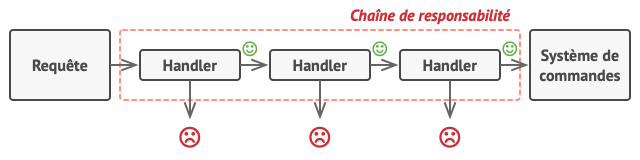
\includegraphics[width=0.6\textwidth]{images/chaine_responsabilité.png}
    \caption{Model de Chaine de responsabilité}
\end{figure}

\section{Répartition des rôles}

La réalisation de ce projet a été organisée de manière collaborative entre les trois membres du groupe. 

Thomas Coutant a principalement travaillé sur le développement du serveur, ainsi que sur la conception de la logique du jeu. Il a également développé un prototype minimal de démarrage, permettant de tester la communication client–serveur avec un simple cube représentant un joueur en mouvement.

Auriane Peter s’est concentrée sur le développement du client, en implémentant l’interface et la gestion des interactions côté joueur.

Benoît Litampha a assuré la communication entre le serveur et le client, participant également à certaines tâches sur le serveur et le client lorsque nécessaire. 

Cette répartition a permis une progression simultanée sur plusieurs fronts du projet, tout en garantissant une cohérence globale de l’application.

%\chapter{L'Organisation du stage}


\chapter{Architecture et conception}

\section{Architecture générale}

Description de l’architecture client-serveur, diagrammes éventuels.

\begin{figure}[H]
    \centering
    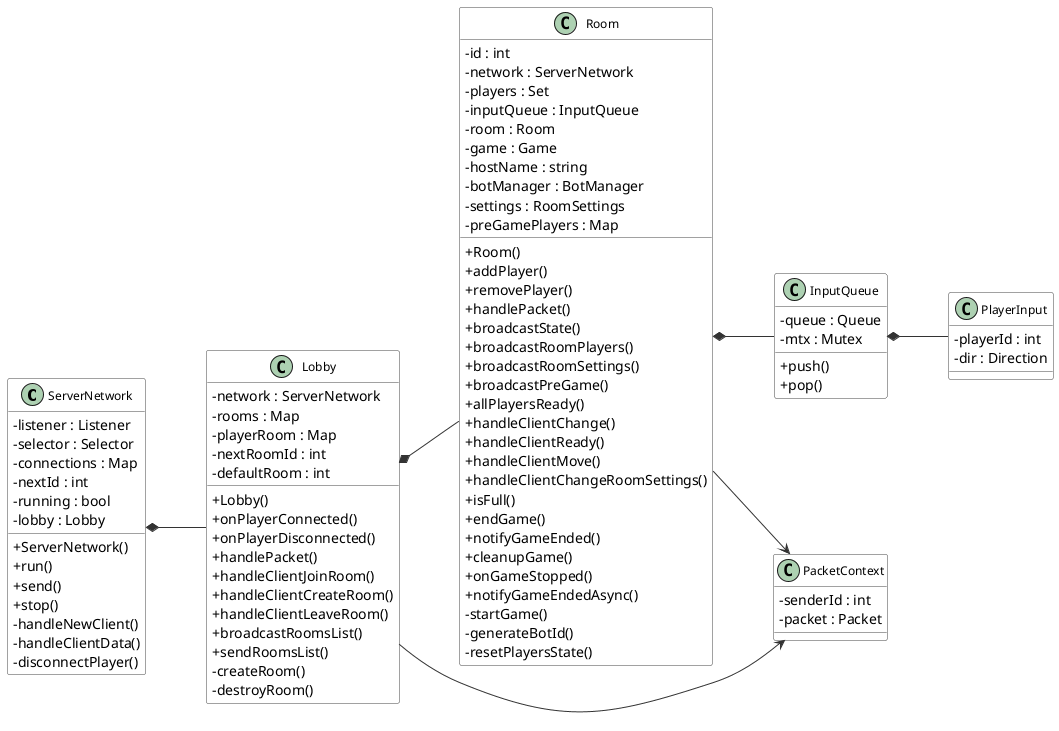
\includegraphics[width=1\textwidth]{UML/PacMan_UML_Server_Reseau.png}
    \caption{Diagrammes de classe de l'architecture réseau}
    \caption*{Vue côté serveur - Gestion des packets, des parties, des salles (sans geter et seter)}

\end{figure}

\section{Structure du serveur}

Gestion des joueurs, des parties, des salles (lobby),
synchronisation de l’état du jeu.

\begin{figure}[H]
    \centering
    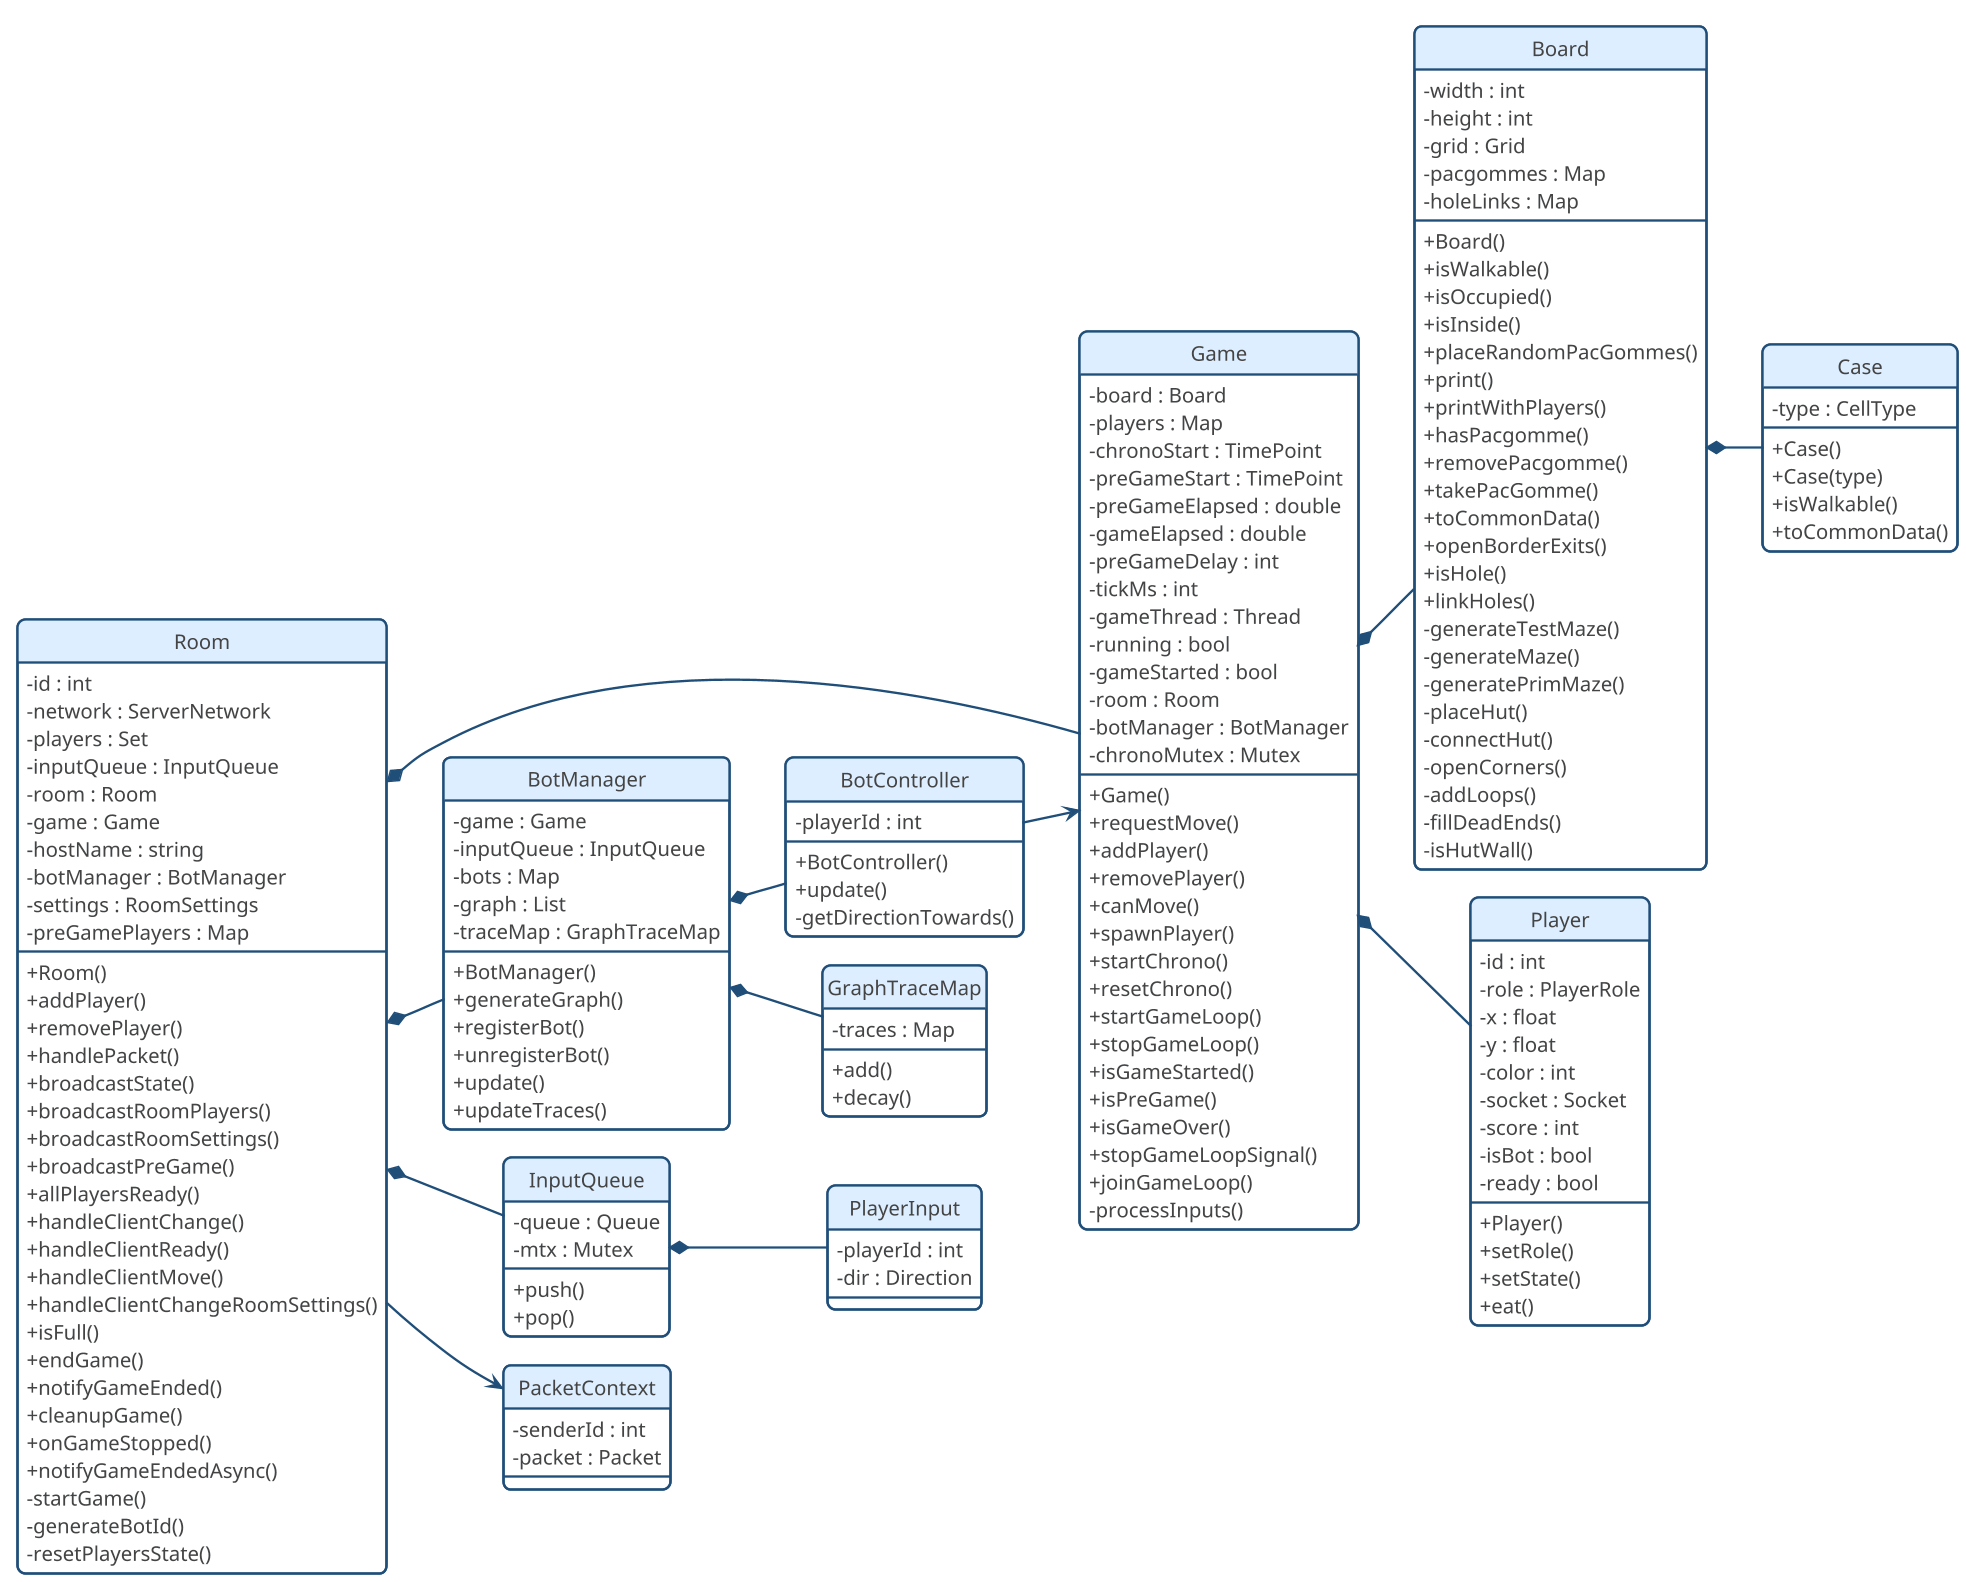
\includegraphics[width=1\textwidth]{UML/PacMan_UML_Server_Game.png}

    \caption{Diagramme de classes de l'architecture de jeu}
    \caption*{Vue côté serveur - synchronisation, rooms et logique de jeu (sans geter et seter)}
\end{figure}


\section{Structure du client}

Affichage, gestion des entrées utilisateur,
réception et traitement des messages réseau.

\section{Protocoles et échanges réseau}

Description des trames, types de messages,
gestion des événements (connexion, mouvement, fin de partie).


Utilisation de gf::TCPSocket, permettant de faire une tramsmission de données fiable
Socket de connnexion + communication coté serveur, communication uniquement pour le client
Un thread coté client et serveur pour empiler les packet reçu, puis dépilement dans la boucle de jeu pour être traité

Structures communes utilisé par le client et serveur pour la communication (BoardCommonn, PlayerData, RoomSettings, etc...)

Sérialisation/Désérialisation avec gf::Packet.is() et gf::Packet.as() et la surchage de | avec la classe Archive. Déjà implémenté pour les types de base par gf

Les structures ont des gf::Id, pour pouvoir les identifier lors de la déserialisation;
Descritpion des strucutres
Exemple avec board : le serveur convertit le plateau en BoardCommon, puis le sérialise avec gf::Packet.is(), avant de l'envoyer au client. Le client traite le packet en regardant si l'id correspond à la structure BoardCommon, puis déserialise avec gf::Packet.as(), avant de traiter les données

Pour chaque modification on retransmet toutes les données


%\section{L'application}

%\section{La gestion des tickets}

\chapter{Réalisation et déroulement du projet}

\section{Mise en place de l’environnement de développement}

\subsection*{Prototype client-serveur initial}

Avant d’implémenter l’ensemble des mécaniques du jeu, une phase de prototypage a été réalisée afin de tester les choix architecturaux initiaux.
L’objectif n’était pas encore de développer un gameplay complet, mais de sécuriser les bases réseau et la synchronisation entre plusieurs clients.

Le prototype consistait en une application minimaliste dans laquelle un client contrôlait le déplacement d’un cube sur un plan 2D. 
Chaque action utilisateur était transmise au serveur sous forme d’intention de déplacement. 
Le serveur recevait cette requête, la validait, mettait à jour l’état interne, puis diffusait la nouvelle position à l’ensemble des clients connectés.

Ce modèle repose sur une architecture dite \textit{serveur autoritaire}. 
Dans cette approche, le serveur est l’unique source de vérité : les clients ne modifient jamais directement l’état du jeu, mais se contentent d’envoyer leurs intentions et d’afficher l’état validé par le serveur.

Ce choix architectural permet de garantir la cohérence globale du système, d’éviter les désynchronisations et de poser des bases solides pour l’extension future vers un véritable jeu multijoueur structuré en rooms et en parties indépendantes.

Ce prototype a ainsi servi de socle technique pour la suite du développement, notamment pour la mise en place du routage des paquets, de la gestion multithread et de la boucle de jeu.

\begin{figure}[H]
    \centering
    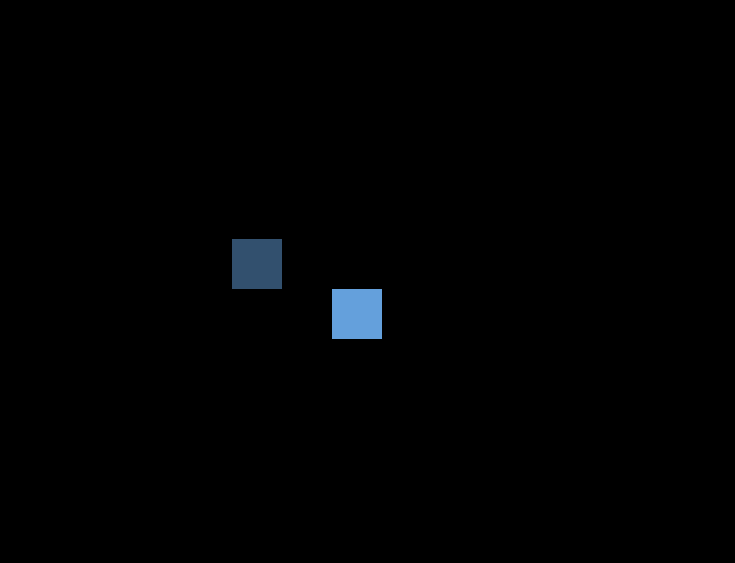
\includegraphics[width=1\textwidth]{images/prototype.png}

    \caption{Premier prototype}
    \caption*{Vue de l'un des clients, il y a 2 client de connecté au serveur}
\end{figure}

\section{Conception de l’architecture du serveur}

Après validation du prototype initial, l’architecture du serveur a été repensée afin de supporter une structure plus complexe adaptée à un jeu multijoueur complet.

L’objectif principal était de passer d’un prototype monolithique à une architecture modulaire, évolutive et maintenable.

\subsection{Mise en place de la structure}

\subsubsection*{Architecture multithread}

Afin de supporter plusieurs connexions simultanées sans dégrader les performances, le serveur repose sur une architecture multithread. 
La gestion réseau est détachée de la logique de jeu afin d’éviter qu’une opération bloquante (attente de paquet, latence réseau, déconnexion) ne ralentisse l’ensemble du système.

Un thread est dédié à la réception des paquets. 
Les messages reçus sont placés dans une file d’attente interne, puis traités de manière synchronisée par la logique centrale du serveur. 
Cette séparation permet de distinguer clairement la couche communication de la couche métier.

L’utilisation de files de messages agit comme un tampon entre le réseau et la boucle de jeu. 
Ainsi, le serveur peut continuer à exécuter ses mises à jour périodiques indépendamment des délais de transmission.

Cette architecture améliore la robustesse du système, limite les risques de blocage et constitue une base adaptée à l’exécution simultanée de plusieurs parties.

\begin{figure}[H]
    \centering
    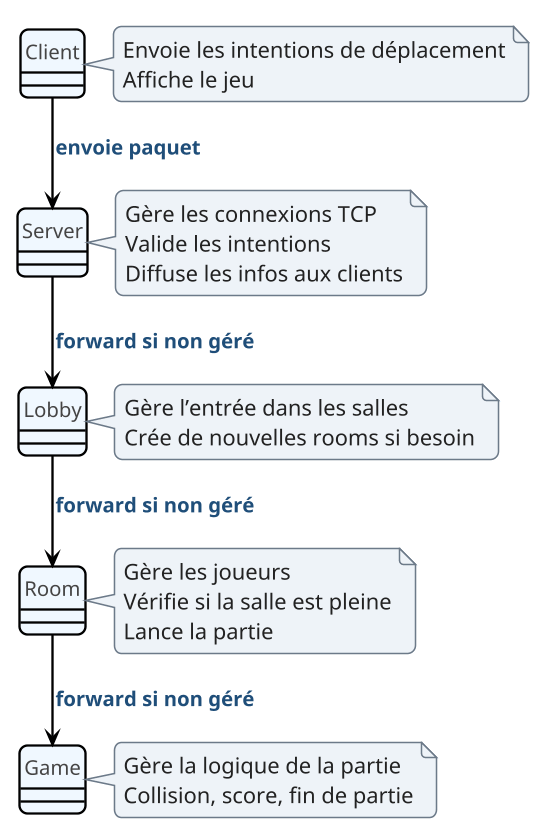
\includegraphics[width=0.6\textwidth]{UML/PacMan_UML_Server_chaine.png}
    \caption{Diagramme de Chaine de responsabilité}
\end{figure}

\subsubsection*{Transformation du prototype}

Le prototype initial validait la communication réseau et le modèle autoritaire, mais son architecture restait monolithique. 
L’ensemble des responsabilités, gestion des connexions, organisation des joueurs et logique de jeu, étaient fortement couplées. 
Cette structure suffisait pour une démonstration technique, mais devenait rapidement limitée dès lors que l’on souhaitait introduire plusieurs parties simultanées.

La transformation du prototype a consisté à structurer le serveur en plusieurs couches distinctes, chacune possédant un rôle clairement défini. 
La gestion réseau a d’abord été isolée de la logique métier afin de rendre le système plus modulaire. 
Un système de \textit{Lobby} a ensuite été introduit pour centraliser la création et l’organisation des parties. 
Chaque partie est encapsulée dans une entité \textit{Room}, responsable de la gestion des joueurs et de leur état avant le démarrage. 
Enfin, la logique complète du jeu est contenue dans une classe dédiée \textit{Game}, indépendante des mécanismes réseau.

L’architecture finale suit ainsi une chaîne de responsabilité structurée :

\begin{center}
    Client $\rightarrow$ Server $\rightarrow$ Lobby $\rightarrow$ Room $\rightarrow$ Game
\end{center}

Chaque couche agit comme un filtre spécialisé qui délègue la responsabilité au niveau inférieur. 
Cette hiérarchisation améliore la lisibilité du code, facilite les tests unitaires et permet d’étendre le système (nouvelles règles, nouveaux modes de jeu) sans modifier la couche réseau.

\subsubsection*{Première implémentation du plateau}

La première version du plateau reposait sur une grille bidimensionnelle composée de cases murales et de cases traversables. 
Cette représentation volontairement simple avait pour objectif de stabiliser le modèle du jeu avant d’introduire des mécanismes plus complexes.

Cette phase intermédiaire a permis de valider plusieurs éléments comme la détection des collisions, la synchronisation des déplacements entre clients et serveur, ainsi que la cohérence entre la représentation logique du plateau côté serveur et son affichage graphique côté client.

Le plateau est ainsi devenu une structure centrale du projet. 
Il ne constituait plus seulement un support visuel, mais une entité logique partagée servant de référence unique pour les calculs de déplacement, la gestion des interactions et, par la suite, pour la génération procédurale du labyrinthe et l’intelligence artificielle des entités ennemies.

\subsection{Mise en place du jeu}

\subsubsection*{Boucle de jeu}

La boucle de jeu constitue le cœur de la logique serveur. 
Contrairement à une architecture purement événementielle, le jeu repose sur un modèle à mise à jour périodique (tick serveur).

Le serveur exécute une boucle principale à intervalle régulier permettant :

\begin{itemize}
    \item De traiter les intentions reçues des clients.
    \item De mettre à jour les positions des entités.
    \item De vérifier les collisions.
    \item De gérer les états temporaires (mode chasseur).
    \item De mettre à jour le score.
    \item De vérifier les conditions de fin de partie.
\end{itemize}

Cette approche garantit que toutes les mises à jour du monde de jeu sont centralisées et synchronisées.\\

\textbf{Rôles des joueurs}\\

Au début de chaque partie, les rôles sont attribués :

\begin{itemize}
    \item Un joueur incarne Pac-Man.
    \item Les autres incarnent des fantômes.
\end{itemize}

Chaque rôle possède des règles de déplacement et de vision spécifiques.\\

\textbf{Gestion des pac-gommes}\\

Le plateau contient deux types de pac-gommes :

\begin{itemize}
    \item Pac-gommes classiques.
    \item Pac-gommes spéciales.
\end{itemize}

Lorsqu’une pac-gomme classique est consommée :
\begin{itemize}
    \item Le score de Pac-Man augmente.
    \item La case devient vide.
\end{itemize}

Lorsqu’une pac-gomme spéciale est consommée :
\begin{itemize}
    \item Pac-Man entre en mode chasseur.
    \item Un timer spécifique est activé.\\
\end{itemize}


\textbf{Gestion du timer}\\

Deux systèmes temporels sont utilisés :

\begin{itemize}
    \item Un timer global de partie.
    \item Un timer temporaire pour le mode chasseur.
\end{itemize}

Le timer global définit la durée maximale d’une partie.
Si celui-ci atteint zéro, la condition de victoire est évaluée.

Le timer du mode chasseur est décrémenté à chaque tick.
Lorsque celui-ci expire, Pac-Man redevient vulnérable.\\

\textbf{Gestion des collisions}\\

Les collisions sont vérifiées à chaque mise à jour :

\begin{itemize}
    \item Collision Pac-Man / mur → déplacement annulé.
    \item Collision Pac-Man / fantôme :
        \begin{itemize}
            \item Si mode normal → perte d’une vie.
            \item Si mode chasseur → fantôme éliminé temporairement.
        \end{itemize}
\end{itemize}

Les collisions sont gérées côté serveur afin d’éviter toute triche ou désynchronisation.\\

\textbf{Synchronisation}\\

À la fin de chaque tick, l’état mis à jour est diffusé à tous les clients via un mécanisme de broadcast.

Ainsi :
\begin{itemize}
    \item Les clients ne calculent jamais la logique.
    \item Ils se contentent d’afficher l’état reçu.
\end{itemize}

\subsubsection*{Plateau et génération procédurale}

Le plateau du jeu repose sur une génération procédurale de labyrinthe.
L’algorithme utilisé est une variante de l’algorithme de Prim appliquée à la génération de labyrinthes.

L’objectif est d’obtenir :

\begin{itemize}
    \item Un labyrinthe connexe.
    \item Une structure cohérente pour le gameplay.
    \item Une forte rejouabilité grâce à la génération aléatoire.
\end{itemize}

\paragraph{Algorithme de génération (variante de Prim)}

Le principe est le suivant :

\begin{enumerate}
    \item Initialisation complète du plateau en murs.
    \item Sélection d’une case initiale (ici $(1,1)$).
    \item Marquage de cette case comme \textit{Floor}.
    \item Ajout des murs voisins dans une liste appelée \textit{frontier}.
\end{enumerate}

Tant que la liste \textit{frontier} n’est pas vide :

\begin{enumerate}
    \item Sélection aléatoire d’un mur dans la frontier.
    \item Vérification s’il possède au moins un voisin déjà marqué comme \textit{Floor}.
    \item Si c’est le cas, suppression du mur entre les deux cases.
    \item Marquage de cette case comme \textit{Floor}.
    \item Ajout de ses voisins encore murs à la frontier.
\end{enumerate}

Ce procédé garantit la création d’un labyrinthe connexe sans îlots isolés.\\

\textbf{Ajout de la cabane centrale}\\

Une zone centrale 3×3, appelée ``cabane'', est insérée au centre du plateau.

Cette zone est protégée durant la génération grâce à une fonction empêchant l’algorithme de Prim de modifier ses murs.

Une fonction \textit{connectHut()} garantit qu’au moins une ouverture relie la cabane au reste du labyrinthe, assurant ainsi son accessibilité.\\

\textbf{Accessibilité des coins}\\

Les coins du plateau sont destinés aux positions initiales des joueurs.
Après génération du labyrinthe, une vérification est effectuée afin de s’assurer que ces zones sont accessibles.

Si nécessaire, des murs adjacents sont ouverts pour relier ces zones au reste du plateau.\\

\textbf{Ajout de cycles}\\

L’algorithme de Prim produit un arbre couvrant, donc un labyrinthe sans cycles.

Afin d’améliorer le gameplay et d’éviter des trajectoires trop prévisibles, des ouvertures supplémentaires sont ajoutées aléatoirement après la génération principale.

Cela permet :

\begin{itemize}
    \item De créer des chemins alternatifs.
    \item D’éviter un comportement trop déterministe.
    \item D’enrichir les stratégies de poursuite.\\
\end{itemize}

\textbf{Suppression des culs-de-sac}\\

Les culs-de-sac sont identifiés en détectant les cases ayant un seul voisin accessible.

Certains sont supprimés en cassant aléatoirement un mur adjacent.
Cela réduit les pièges trop défavorables pour Pac-Man et améliore la fluidité du jeu.\\

\textbf{Portails}\\

Des ouvertures spécifiques sont placées sur les bords du plateau afin de créer des portails.
Ces passages permettent à une entité sortant d’un côté du plateau de réapparaître de l’autre côté.

Ce mécanisme introduit :

\begin{itemize}
    \item Des stratégies d’évasion supplémentaires.
    \item Une dynamique de poursuite plus complexe.\\
\end{itemize}

\textbf{Intégration gameplay}\\

Le plateau devient ainsi une structure centrale du système :

\begin{itemize}
    \item Support de la logique de collision.
    \item Support du pathfinding des fantômes.
    \item Support du placement des pac-gommes.
\end{itemize}

La génération procédurale contribue fortement à la rejouabilité et à la variabilité stratégique des parties.

\subsubsection{Intelligence artificielle des fantômes}

L’intelligence artificielle des fantômes repose sur une architecture hybride combinant :

\begin{itemize}
    \item Pathfinding classique
    \item Système d’influence inspiré des colonies de fourmis
    \item Prise de décision hiérarchique
\end{itemize}

L’objectif est d’obtenir un comportement :

\begin{itemize}
    \item Réactif face aux situations critiques
    \item Cohérent dans ses déplacements
    \item Émergent lorsqu’il y a plusieurs fantômes
\end{itemize}

\paragraph{Architecture décisionnelle hiérarchique}

Le système fonctionne par niveaux de priorité.
À chaque tick serveur, le fantôme évalue sa situation selon l’ordre suivant :

\subparagraph{Priorité 1 — Fuite stratégique}

Si Pac-Man est en mode chasseur, le fantôme cherche à rejoindre la cabane centrale.

Pour cela, un algorithme de \textbf{Breadth First Search (BFS)} est utilisé afin d’obtenir le plus court chemin non pondéré.

Le BFS garantit :
\begin{itemize}
    \item Un chemin optimal
    \item Une complexité maîtrisée
    \item Une robustesse face aux labyrinthes générés procéduralement
\end{itemize}

\subparagraph{Priorité 2 — Poursuite ciblée}

Si Pac-Man est détecté dans un rayon de vision défini :

\begin{itemize}
    \item Un BFS à profondeur limitée est exécuté.
    \item Le voisin rapprochant le plus rapidement de la cible est sélectionné.
\end{itemize}

Cette limitation permet :
\begin{itemize}
    \item De simuler une vision partielle.
    \item De réduire le coût computationnel.
\end{itemize}

\subparagraph{Priorité 3 — Comportement autonome}

En absence de menace ou de cible visible, le fantôme adopte un comportement autonome basé sur un système d’influence.

\paragraph{Système d’influence}

Chaque case du plateau possède un score calculé dynamiquement :

\[
Score = Attraction - Répulsions
\]

Les composantes sont les suivantes :

\begin{itemize}
    \item Traces de Pac-Man $\rightarrow$ Attraction
    \item Traces de fantômes alliés $\rightarrow$ Répulsion forte
    \item Traces de fantômes adverses $\rightarrow$ Répulsion modérée
\end{itemize}

Le fantôme sélectionne le voisin présentant le score maximal.
Il s’agit d’une approche locale de type \textit{greedy search}.

\paragraph{Comportement émergent}

Ce système permet l’émergence de comportements collectifs naturels :

\begin{itemize}
    \item Dispersion automatique des fantômes
    \item Réduction des regroupements inutiles
    \item Convergence progressive vers Pac-Man
\end{itemize}

Sans coordination explicite entre les agents, un équilibre dynamique apparaît.

\paragraph{Techniques utilisées}

L’implémentation repose sur plusieurs techniques algorithmiques :

\begin{itemize}
    \item \textbf{Breadth First Search (BFS)} — plus court chemin
    \item \textbf{BFS limité} — simulation de vision
    \item \textbf{Recherche gloutonne locale} — sélection optimale immédiate
    \item \textbf{Distance euclidienne au carré} — heuristique rapide
    \item \textbf{Bruit aléatoire contrôlé} — prévention des cycles et oscillations
\end{itemize}

L’approche hybride permet d’obtenir un compromis entre précision stratégique et coût computationnel maîtrisé.

\subsubsection{Rooms : gestion des parties}

Afin de supporter plusieurs parties simultanées, le serveur utilise un système de \textbf{rooms}. 
Chaque room est un espace indépendant qui gère :

\begin{itemize}
    \item La liste des joueurs connectés
    \item Les rôles attribués à chaque joueur (Pac-Man ou fantôme)
    \item Les paramètres de la partie (durée, nombre de vies, nombre de pac-gommes spéciales)
    \item L’état de la partie (en attente, en cours, terminée)
\end{itemize}

\paragraph{Création et attribution des rôles}

\begin{itemize}
    \item Lorsqu’un joueur rejoint un lobby, il peut entrer dans une room disponible.
    \item Si aucune room n’est disponible, une nouvelle room est créée automatiquement.
    \item Les rôles sont assignés en fonction des règles :
    \begin{itemize}
        \item Un joueur est choisi comme Pac-Man
        \item Les autres sont des fantômes
    \end{itemize}
\end{itemize}

\paragraph{Transmission des informations}

Chaque room maintient un état centralisé, qui est diffusé à tous les joueurs connectés via le serveur :

\begin{itemize}
    \item Position des joueurs
    \item État des pac-gommes
    \item État des timers (partie et mode chasseur)
\end{itemize}

Cette approche garantit :

\begin{itemize}
    \item La cohérence des parties multijoueurs
    \item L’isolation des parties entre elles
    \item Une architecture modulaire et scalable
\end{itemize}

\paragraph{Paramètres de la partie}

Les rooms permettent de configurer :

\begin{itemize}
    \item La durée de la partie
    \item Le nombre de vies de Pac-Man
    \item Le nombre et la disposition des pac-gommes spéciales
\end{itemize}

Ainsi, chaque partie peut avoir des règles légèrement différentes, offrant plus de rejouabilité et de flexibilité pour les tests et la compétition entre joueurs.

\subsubsection{Règles du jeu}

Le jeu respecte des règles spécifiques pour Pac-Man et les fantômes, afin de garantir un gameplay équilibré et stratégique.

\paragraph{Conditions de victoire}

\begin{itemize}
    \item \textbf{Pour Pac-Man} : 
    \begin{itemize}
        \item Avoir consommé toutes les pac-gommes du plateau
        \item Ou survivre jusqu’à la fin du timer de la partie
    \end{itemize}
    \item \textbf{Pour les fantômes} :
    \begin{itemize}
        \item Éliminer Pac-Man en lui faisant perdre toutes ses vies
    \end{itemize}
\end{itemize}

\paragraph{Pac-gommes spéciales}

Certaines pac-gommes permettent à Pac-Man d’entrer temporairement en \textit{mode chasseur} :

\begin{itemize}
    \item Pendant cette période, Pac-Man peut éliminer les fantômes.
    \item La durée du mode est limitée par un timer spécifique.
    \item Les fantômes affectés réapparaissent après un certain délai.
\end{itemize}

\paragraph{Vision des joueurs}

\begin{itemize}
    \item Les fantômes ne voient qu’autour d’eux (vision locale limitée).
    \item Pac-Man voit l’ensemble du plateau.
\end{itemize}

Cette asymétrie introduit une dynamique de jeu intéressante et stratégique :

\begin{itemize}
    \item Les fantômes doivent coopérer pour localiser Pac-Man.
    \item Pac-Man peut planifier ses déplacements en connaissance de cause.
\end{itemize}

\paragraph{Résumé du système}

La combinaison de ces règles avec la génération procédurale et l’IA des fantômes permet :

\begin{itemize}
    \item Un gameplay varié et imprévisible.
    \item La possibilité pour Pac-Man et les fantômes de développer des stratégies différentes.
    \item Une forte rejouabilité du jeu.
\end{itemize}

\chapter{Bilan et perspectives}

\section{Compétences acquises}

Programmation réseau, architecture logicielle,
travail de conception.

\section{Résultat final}

Fonctionnalités implémentées,
objectifs atteints ou partiellement atteints.

\section{Améliorations possibles}

idee.txt



% Page de conclusion 
\chapter*{Conclusion}
\addcontentsline{toc}{chapter}{Conclusion}

Ce projet a permis de mettre en pratique les connaissances acquises
durant la formation en informatique, en particulier dans le domaine
du développement réseau et de la conception logicielle.




% Page de conclusion 
\chapter*{Sitographie}
\addcontentsline{toc}{chapter}{Sitographie} % Ajout de la sitographie sur la table des matières sans ètre numéroté


% Page de résumé
\newpage
\begin{center}
    \vspace*{\fill} % Espace vertical
    \section*{Résumé}
    \addcontentsline
    {toc}{chapter}{Résumé}
    \begin{justify}

    \end{justify}
    \vspace*{\fill} % Espace vertical

    \section*{Mots-clés}
    \addcontentsline
    {toc}{chapter}{Mots-Clés}
    \begin{center}
     C++ - PacMan - GF - Réseau - [AUTRE]
    \end{center}
    \vspace*{\fill} % Espace vertical

    \section*{Abstract}
    \addcontentsline
    {toc}{chapter}{Abstract}
    \begin{justify}

    \end{justify}
    \vspace*{\fill} % Espace vertical

    \section*{Key-Words}
    \addcontentsline
    {toc}{chapter}{Key-Words}
    \begin{center}
    MathLive - JavaScript - TypeScript - HTML - Drag \& Drop
    \end{center}
    \vspace*{\fill} % Espace vertical
    
    
\end{center}

\end{document}